\documentclass{article}

    \usepackage{fancyhdr}
    \usepackage{extramarks}
    \usepackage{amsmath}
    \usepackage{amsthm}
    \usepackage{amsfonts}
    \usepackage{tikz}
    \usepackage{amssymb}
    \usepackage{subcaption}
    \usepackage{blkarray}
    \usetikzlibrary{arrows, automata}
    \usepackage{forest}
    
    \usetikzlibrary{trees}
    


    \usetikzlibrary{decorations.markings}
    \tikzstyle{vertex}=[circle, draw, inner sep=0pt, minimum size=6pt]
    \newcommand{\vertex}{\node[vertex]}

    
    \usepackage{amsmath}
    \usepackage{algorithm}
    \usepackage[noend]{algpseudocode}
    \usepackage[utf8]{inputenc}
    \usepackage{enumerate}
    \usepackage{geometry}
    \usepackage{mathtools}
    \usepackage{parskip}
    \usepackage{xifthen, xparse}
    
    \algdef{SE}[SUBALG]{Indent}{EndIndent}{}{\algorithmicend\ }%
    \algtext*{Indent}
    \algtext*{EndIndent}
    
    
    
    \usetikzlibrary{automata,positioning}
    
    %
    % Basic Document Settings
    %
    
    \topmargin=-0.45in
    \evensidemargin=0in
    \oddsidemargin=0in
    \textwidth=6.5in
    \textheight=9.0in
    \headsep=0.25in
    
    \linespread{1.1}
    
    \pagestyle{fancy}
    \lhead{\hmwkAuthorName}
    \chead{\hmwkClass\ \hmwkTitle}
    \rhead{\firstxmark}
    \lfoot{\lastxmark}
    \cfoot{\thepage}
    
    \renewcommand\headrulewidth{0.4pt}
    \renewcommand\footrulewidth{0.4pt}
    
    \setlength\parindent{0pt}
    
    %
    % Create Problem Sections
    %
    
    \newcommand{\enterProblemHeader}[1]{
        \nobreak\extramarks{}{Problem \arabic{#1} continued on next page\ldots}\nobreak{}
        \nobreak\extramarks{Problem \arabic{#1} (continued)}{Problem \arabic{#1} continued on next page\ldots}\nobreak{}
    }
    
    \newcommand{\exitProblemHeader}[1]{
        \nobreak\extramarks{Problem \arabic{#1} (continued)}{Problem \arabic{#1} continued on next page\ldots}\nobreak{}
        \stepcounter{#1}
        \nobreak\extramarks{Problem \arabic{#1}}{}\nobreak{}
    }
    
    \newcommand\rowop[1]{\scriptstyle\smash{\xrightarrow[\vphantom{#1}]{\mkern-4mu#1\mkern-4mu}}}
    
    \DeclareDocumentCommand\converttorows%
    {>{\SplitList{,}}m}%
    {\ProcessList{#1}{\converttorow}}
    \NewDocumentCommand{\converttorow}{m}
    {\ifthenelse{\isempty{#1}}{}{\rowop{#1}}\\}
    
    \DeclareDocumentCommand \rowops{m}
    {\;
     \begin{matrix}
    \converttorows {#1}
     \end{matrix}
     \; }
    
    \setcounter{secnumdepth}{0}
    \newcounter{partCounter}
    \newcounter{homeworkProblemCounter}
    \setcounter{homeworkProblemCounter}{1}
    \nobreak\extramarks{Problem \arabic{homeworkProblemCounter}}{}\nobreak{}
    
    %
    % Homework Problem Environment
    %
    % This environment takes an optional argument. When given, it will adjust the
    % problem counter. This is useful for when the problems given for your
    % assignment aren't sequential. See the last 3 problems of this template for an
    % example.
    %
    \newenvironment{homeworkProblem}[1][-1]{
        \ifnum#1>0
            \setcounter{homeworkProblemCounter}{#1}
        \fi
        \section{Problem \arabic{homeworkProblemCounter}}
        \setcounter{partCounter}{1}
        \enterProblemHeader{homeworkProblemCounter}
    }{
        \exitProblemHeader{homeworkProblemCounter}
    }
    
    %
    % Homework Details
    %   - Title
    %   - Due date
    %   - Class
    %   - Section/Time
    %   - Instructor
    %   - Author
    %
    
    \newcommand{\hmwkTitle}{SOFTENG250 Assignment \#4}
    \newcommand{\hmwkClass}{D.S. and Algorithms}
    \newcommand{\hmwkAuthorName}{\textbf{Nisarag Bhatt}}
    
    
    %
    % Title Page
    %
    
    \title{
        \vspace{2in}
        \textmd{\textbf{\hmwkClass:\ \hmwkTitle}}\\
        \textmd{\textbf{ID Number: \idnumber}}\\
        \textmd{\textbf{UPI: \upi}}\\
        \vspace{3in}
    }
    
    \author{\hmwkAuthorName}
    \date{}
    
    \renewcommand{\part}[1]{\textbf{\large Part \Alph{partCounter}}\stepcounter{partCounter}\\}
    
    %
    % Various Helper Commands
    %
    
    % Useful for algorithms
    \newcommand{\alg}[1]{\textsc{\bfseries \footnotesize #1}}
    
    % For derivatives
    \newcommand{\deriv}[1]{\frac{\mathrm{d}}{\mathrm{d}x} (#1)}
    
    % For partial derivatives
    \newcommand{\pderiv}[2]{\frac{\partial}{\partial #1} (#2)}
    
    % Integral dx
    \newcommand{\dx}{\mathrm{d}x}
    
    % Alias for the Solution section header
    \newcommand{\solution}{\textbf{\large Solution}}
    
    % Probability commands: Expectation, Variance, Covariance, Bias
    \newcommand{\E}{\mathrm{E}}
    \newcommand{\Var}{\mathrm{Var}}
    \newcommand{\Cov}{\mathrm{Cov}}
    \newcommand{\Bias}{\mathrm{Bias}}
    
    \begin{document}
    
    
    \pagebreak
    
    \begin{homeworkProblem}
    
        \textbf{Question}: Suppose the selection rule for the interval scheduling problem is the following. Select a request that has the fewest possible requests overlapping it. Give an example where this rule does not provide an optimal solution. 
        
        \textbf{Solution:} 

        Consider these requests at certain times:

        \begin{tikzpicture}
            \draw (0,0) -- (2.8,0)  node[above,xshift=-1.4cm] {$r_1$};
            \draw (3.1,0) -- (5.9,0) node[above,xshift=-1.4cm] {$r_2$};
            \draw (6.2,0) -- (9,0) node[above,xshift=-1.4cm] {$r_3$};
            \draw (9.3,0) -- (12.1,0) node[above,xshift=-1.4cm] {$r_4$};
            \draw (2.4,-0.7) -- (3.4,-0.7) node[above,xshift=-0.5cm] {$r_5$};
            \draw (5.5,-0.7) -- (7.5,-0.7) node[above,xshift=-1cm] {$r_6$};
            \draw (8.5,-0.7) -- (10,-0.7) node[above,xshift=-0.75cm] {$r_7$};
            \draw (2.4,-1.4) -- (3.4,-1.4) node[above,xshift=-0.5cm] {$r_8$};
            \draw (8.47,-1.4) -- (9.97,-1.4) node[above,xshift=-0.75cm] {$r_9$};
            \draw (2.4,-2.1) -- (3.4,-2.1) node[above,xshift=-0.5cm] {$r_{11}$};
            \draw (8.5,-2.1) -- (10,-2.1) node[above,xshift=-0.75cm] {$r_{12}$};
        \end{tikzpicture}

        The greedy method suggested here accepts the middle request in the second row ($r_6$) and thereby ensures a solution of size no greater than three.

        However the optimal solution in this example is to accept the four requests in the top row. 
    \end{homeworkProblem}

    \begin{homeworkProblem}
        \textbf{Question}: Find a necessary and sufficient condition on $n$ requests that guarantees that any optimal solution to the interval colouring problem would require $n$ resources.

        \textbf{Solution}: If the requests are pairwise incompatible, then none of the requests can scheduled on the same resource, thus $n$ requests will require $n$ resources.
    \end{homeworkProblem}

    \begin{homeworkProblem}
        \textbf{Question}: Explain an algorithm for the interval colouring problem that runs in $O(n \cdot \log(d))$ time. Here you just need to say what data structure you would use, describe your data structure and explain why you would achieve the bound. Keep your answer compact.

        \textbf{Solution}: To ensure the runtime of our algorithm is $O(n \cdot \log(d))$ we can use a heap to store our resources.

        The key of the resources is the finishing time of the last request assigned to the resource. The minimum finishing time is given the highest priority. 
        
        There are $n$ requests, so $n$ iterations, one for each request, and in each iteration, the highest priority resource is picked, this takes constant time.

        Through the algorithm:

        \begin{enumerate}
            \item The request is compatible with the resource, it is assigned to the resource. The request now has a later/larger finishing time, so we run heapify-down on the resource, this takes $O(\log d)$ time.
            \item The request is incompatible with the resource, and thus all the other resources. So, a new resource is created, and the request is assigned to the new resource. The resource is inserted into the heap, which takes $O(\log d)$ time.
        \end{enumerate}

        Therefore since there are $n$ iterations, and each iteration has a running time of $\log(d)$ we have that the overall run time is $O(n \cdot \log(d))$
    \end{homeworkProblem}

    \begin{homeworkProblem}
        \textbf{Question}: Solve Exercise 2 from Lecture Note 8.

        \textbf{Answer}:
        \begin{itemize}
            \item Schedule those requests that occupy the resources the shortest amount of time.
            \begin{itemize}
                \item Consider the case when we have two requests (in the form $R=[t_i, d_i]$) $R_1 =[1,15] $, $R_2=[10,10]$, This algorithm schedules $R_1$ first then $R_2$ and thus results in a maximum lateness of $1$, while scheduling $R_2$ first then $R_1$ gives a maximum lateness of $0$ (which is optimal in this case). 
            \end{itemize}
            \item Schedule those requests that have the least slack time.
            \begin{itemize}
                \item Consider the case when we have two requests (in the form $R=[t_i, d_i, \text{slack}_i]$) $R_1=[1,2,1]$, $R_2=[10,10,0]$.
                This algorithm schedules $R_2$ first as it has $0$ slack then $R_1$ which means that our maximum lateness is 9. However the optimal solution would schedule $R_1$ first then $R_2$ which has a maximum lateness of $1$.
            \end{itemize}
        \end{itemize}

    \end{homeworkProblem}

    \begin{homeworkProblem}
        \textbf{Question}: Solve Exercises 1,2,3 from Lecture Note 9.

        \begin{itemize}
            \item Exercise 1: 
                \begin{itemize}
                    \item From vertex $e$ to $x$ the shortest path is $e \to w \to y \to q \to z \to x$ with a weight of $13$
                    \item From vertex $a$ to $y$ the shortest path is $a \to b \to f \to u \to w \to y$ with a weight of $9$ 
                \end{itemize}
            \item Exercise 2:
                \begin{itemize}
                    \item If there is one path from $u$ to $v$ then the weight of path is minimal so we are done since it is the shortest. Suppose there are $k$ paths from $u$ to $v$ then we pick the one with minimal weight and that is the shortest one so we are done.
                \end{itemize}
            \item Exercise 3:
                \begin{itemize}
                    \item If we consider this image
                \end{itemize}
        \end{itemize}



        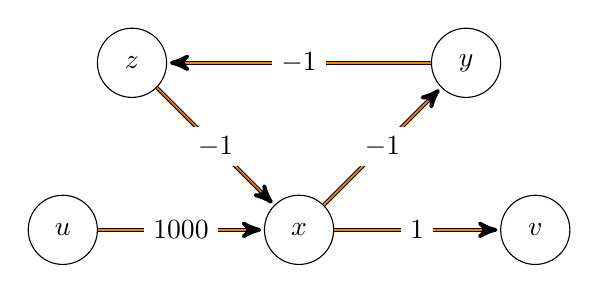
\begin{tikzpicture}[>=stealth',shorten >=1pt,node distance=3cm,on grid,initial/.style    ={}]
            \node[state]          (u)                        {$u$};
            \node[state]          (x) [right =of u]    {$x$};
            \node[state]          (z) [above left =of x]    {$z$};
            \node[state]          (y) [above right =of x]    {$y$};
            \node[state]          (v) [right =of x]    {$v$};
            \tikzset{mystyle/.style={->,double=orange}} 
            \tikzset{every node/.style={fill=white}} 
            \path (u)     edge [mystyle]    node   {$1000$} (x);
            \path (x)     edge [mystyle]    node   {$-1$} (y);
            \path (y)     edge [mystyle]    node   {$-1$} (z);
            \path (z)     edge [mystyle]    node   {$-1$} (x);
            \path (x)     edge [mystyle]    node   {$1$} (v);
        \end{tikzpicture}

        Then we can take the path $u \to x \to v$ which has cost $1001$, or we can take the path $u \to x \to y \to z \to x \to v$ which has cost $998$, or we can take the path $u \to x \to y \to z \to x \to y \to z \to x \to v$ which has cost $995$ hence even though there is a path from $u$ to $v$ we cannot determine if the shortest path exists from $u$ to $v$ since we can keep going through the cycle $x \to y \to z$ to keep reducing the path cost.
    \end{homeworkProblem}




    \end{document}
    